\section{Volumi di solidi regolari}
\subsection{Cubo}
Il cubo è un solido con 6 facce quadrate congruenti.

\begin{figure}[!htbp] 
\centering
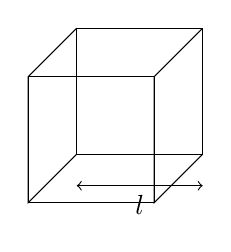
\begin{tikzpicture}[scale=0.8]
    \draw (0,0,0) -- (2,0,0) -- (2,2,0) -- (0,2,0) -- cycle;
    \draw (0,0,0) -- (0,0,2) -- (0,2,2) -- (0,2,0);
    \draw (2,0,0) -- (2,0,2) -- (2,2,2) -- (2,2,0);
    \draw (0,0,2) -- (2,0,2) -- (2,2,2) -- (0,2,2) -- cycle;
    \draw[<->] (0,-0.5,0) -- node[below] {$l$} (2,-0.5,0);
\end{tikzpicture}
\caption{Cubo con lato $l$}
\end{figure}

\textbf{Formula del volume:} $V = l^3$

\subsection{Parallelepipedo}
Il parallelepipedo è un solido con 6 facce rettangolari.

\begin{figure}[!htbp] 
\centering
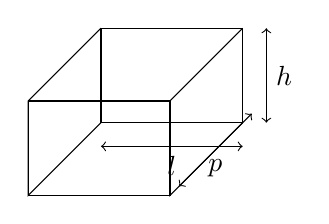
\begin{tikzpicture}[scale=0.6]
    \draw (0,0,0) -- (3,0,0) -- (3,2,0) -- (0,2,0) -- cycle;
    \draw (0,0,0) -- (0,0,4) -- (0,2,4) -- (0,2,0);
    \draw (3,0,0) -- (3,0,4) -- (3,2,4) -- (3,2,0);
    \draw (0,0,4) -- (3,0,4) -- (3,2,4) -- (0,2,4) -- cycle;
    \draw[<->] (0,-0.5,0) -- node[below] {$l$} (3,-0.5,0);
    \draw[<->] (3.5,0,0) -- node[right] {$h$} (3.5,2,0);
    \draw[<->] (3,0,-0.5) -- node[below] {$p$} (3,0,3.5);
\end{tikzpicture}
\caption{Parallelepipedo con dimensioni $l$, $h$, $p$}
\end{figure}

\textbf{Formula del volume:} $V = l \cdot h \cdot p$

\subsection{Cilindro}
Il cilindro è un solido generato dalla rotazione di un rettangolo attorno a uno dei suoi lati.

\begin{figure}[!htbp] 
\centering
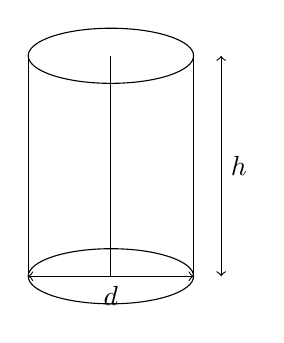
\begin{tikzpicture}[scale=0.7]
    % Disegna le ellissi
    \draw (0,0) ellipse (1.5cm and 0.5cm);
    \draw (0,4) ellipse (1.5cm and 0.5cm);
    % Disegna le linee verticali
    \draw (-1.5,0) -- (-1.5,4);
    \draw (1.5,0) -- (1.5,4);
    % Disegna le linee laterali
    \draw (0,0) -- (0,4);
    % Disegna le linee di misurazione
    \draw[<->] (-1.5,0) -- node[below] {$d$} (1.5,0);
    \draw[<->] (2,0) -- node[right] {$h$} (2,4);
\end{tikzpicture}
\caption{Cilindro con diametro $d$ e altezza $h$}
\end{figure}

\textbf{Formula del volume:} $V = \frac{\pi d^2}{4} \cdot h$

\subsection{Cono a base retta}
Il cono a base retta è un solido generato dalla rotazione di un triangolo rettangolo attorno a uno dei suoi cateti.

\begin{figure}[!htbp] 
\centering
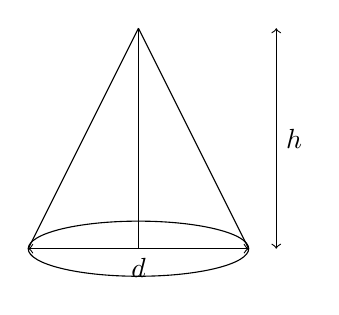
\begin{tikzpicture}[scale=0.7]
    \draw (0,0) ellipse (2cm and 0.5cm);
    \draw (0,0) -- (0,4);
    \draw (2,0) -- (0,4);
    \draw (-2,0) -- (0,4);
    \draw[dashed] (0,0) -- (2,0);
\draw[<->] (-2,0) -- node[below] {$d$} (2,0);
    \draw[<->] (2.5,0) -- node[right] {$h$} (2.5,4);
\end{tikzpicture}
\caption{Cono con diametro $d$ e altezza $h$}
\end{figure}

\textbf{Formula del volume:} $V = \frac{\pi d^2}{12} \cdot h$

\subsection{Sfera}
La sfera è un solido generato dalla rotazione di un semicerchio attorno al suo diametro.

\begin{figure}[!htbp] 
\centering
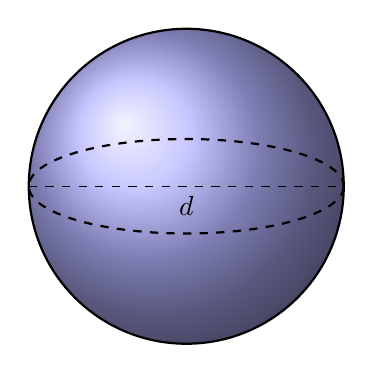
\begin{tikzpicture}[scale=1]
    % Disegna la sfera con sfumatura
    \shade[ball color=blue!30] (0,0) circle (2cm);
    % Disegna l'equatore con linea continua
    \draw[dashed, thick] (0,0) ellipse (2cm and 0.6cm);

    % Disegna il contorno della sfera
    \draw[thick] (0,0) circle (2cm);

    % Disegna il diametro orizzontale tratteggiato
    \draw[dashed] (-2,0) -- (2,0);

    % Etichetta del diametro
    \node[below] at (0,0) {$d$};
\end{tikzpicture}
\caption{Sfera.}
\end{figure}

\textbf{Formula del volume:} $V = \frac{\pi d^3}{6}$

\subsection{Esercizi svolti}

\eserciziop{Calcola il volume di un cubo con lato \SI{5,00}{\centi\metre}.}

\soluzione{
$V = l^3 = (\SI{5}{\centi\metre})^3 = \SI{125}{\centi\metre\cubed}$
}

\eserciziop{Calcola il volume di un parallelepipedo con lunghezza \SI{6,0}{\centi\metre}, larghezza \SI{4,0}{\centi\metre} e altezza \SI{3,0}{\centi\metre}.}

\soluzione{
$V = l \cdot h \cdot p = \SI{6}{\centi\metre} \cdot \SI{4}{\centi\metre} \cdot \SI{3}{\centi\metre} = \SI{72}{\centi\metre\cubed}$
}

\eserciziop{Calcola il volume di un cilindro con diametro \SI{8,00000}{\centi\metre} e altezza \SI{10,000}{\centi\metre}.}

\soluzione{
$V = \frac{\pi d^2}{4} \cdot h = \frac{\pi \cdot (\SI{8}{\centi\metre})^2}{4} \cdot \SI{10}{\centi\metre} \approx \SI{502,65}{\centi\metre\cubed}$
}

\eserciziop{Calcola il volume di un cono a base retta con diametro \SI{6,000}{\centi\metre} e altezza \SI{9,000}{\centi\metre}.}

\soluzione{
$V = \frac{\pi d^2}{12} \cdot h = \frac{\pi \cdot (\SI{6}{\centi\metre})^2}{12} \cdot \SI{9}{\centi\metre} \approx \SI{84,82}{\centi\metre\cubed}$
}

\eserciziop{Calcola il volume di una sfera con diametro \SI{10,000}{\centi\metre}.}

\soluzione{
$V = \frac{\pi d^3}{6} = \frac{\pi \cdot (\SI{10}{\centi\metre})^3}{6} \approx \SI{523,60}{\centi\metre\cubed}$
}


